\documentclass[10pt]{beamer}
%\usepackage[utf8]{inputenc}
\usepackage[T1]{fontenc}
\usepackage{lmodern}
\usetheme{focus}
\usepackage{xcolor}
\usepackage[ngerman]{babel}
\usepackage{graphicx}

\definecolor{main}{RGB}{30, 30, 46}
\definecolor{background}{RGB}{255, 255, 255}    
\setbeamerfont{title}{size=\LARGE}
\setbeamerfont{caption}{size=\small}
\AtBeginSection{}

\begin{document}
	\author{\small Ayleen Edenhauser,
				   Matteo Volperino,
				   Jakob Oberhofer,
				   Leonid Stommel }
			% Das ist eine unsaubere Lösung und produziert eine Warnung
	\title{The Retro Duck
		\\Unser Retro Gaming Shop (mit Enten)}
	\subtitle{Projekt für Softwarearchitektur}
	\institute{\small Universität Innsbruck}
	\date{\small \today, RR15}
	
	%\setbeamercovered{transparent}
	%\setbeamertemplate{navigation symbols}{}
	\begin{frame}[plain]
		\titlepage
		\begin{minipage}{0.6\textwidth}
			\small
			PS Softwarearchitektur WS 2025/26 
			
		\end{minipage}
		\hfill
		\begin{minipage}{0.35\textwidth}
			\begin{flushright}
			
\includegraphics[width=3.0cm]{universitaet-innsbruck-logo-cmyk-farbe.jpg}
			\end{flushright}
		\end{minipage}
	\end{frame}
	
	\begin{frame}
		\frametitle{Überblick}
		\tableofcontents
	\end{frame}
	
\section{Planung und Projektmanagement}
\begin{frame}
	\frametitle{Planung und Projektmanagement}
	\begin{minipage}{0.55\textwidth}
		\begin{itemize}
			\item UML für Backend-Design wichtig
			\item Zeiteinschätzung war nicht akkurat... aber machbar!
			\item Frontend und Debugging (API-Schnittstelle) hat am meisten Zeit gekostet
			\item Projektplan als Überblick
			\item Wöchtentliche Merge Requests
			\item Aufteilung: Full Stack - Ein Feature pro Person
			\item Jeder konnte unabhängig arbeiten. Produkte waren die größte Dependency
		\end{itemize}
	\end{minipage}
	\hfill
	\begin{minipage}{0.35\textwidth}
		\begin{figure}
			\raggedright
			
\includegraphics[width=\textwidth]{1}
		\end{figure}
	\end{minipage}
\end{frame}

\section{Technologie}
\begin{frame}
	\frametitle{Technologie}
	\begin{minipage}{0.4\textwidth}
		\begin{itemize}
			\item Spring macht Java besser!
			\item Nützlich für Entitäten, Observer, Singleton uvm.
			\item React ist sehr angenehm. Doku > ChatGPT
			\item CSS Styling!
			\item KI wurde für Dummy Testdaten und Frontend Layout genutzt
		\end{itemize}
	\end{minipage}
	\hfill
	\begin{minipage}{0.5\textwidth}
		\begin{figure}
			\raggedright
			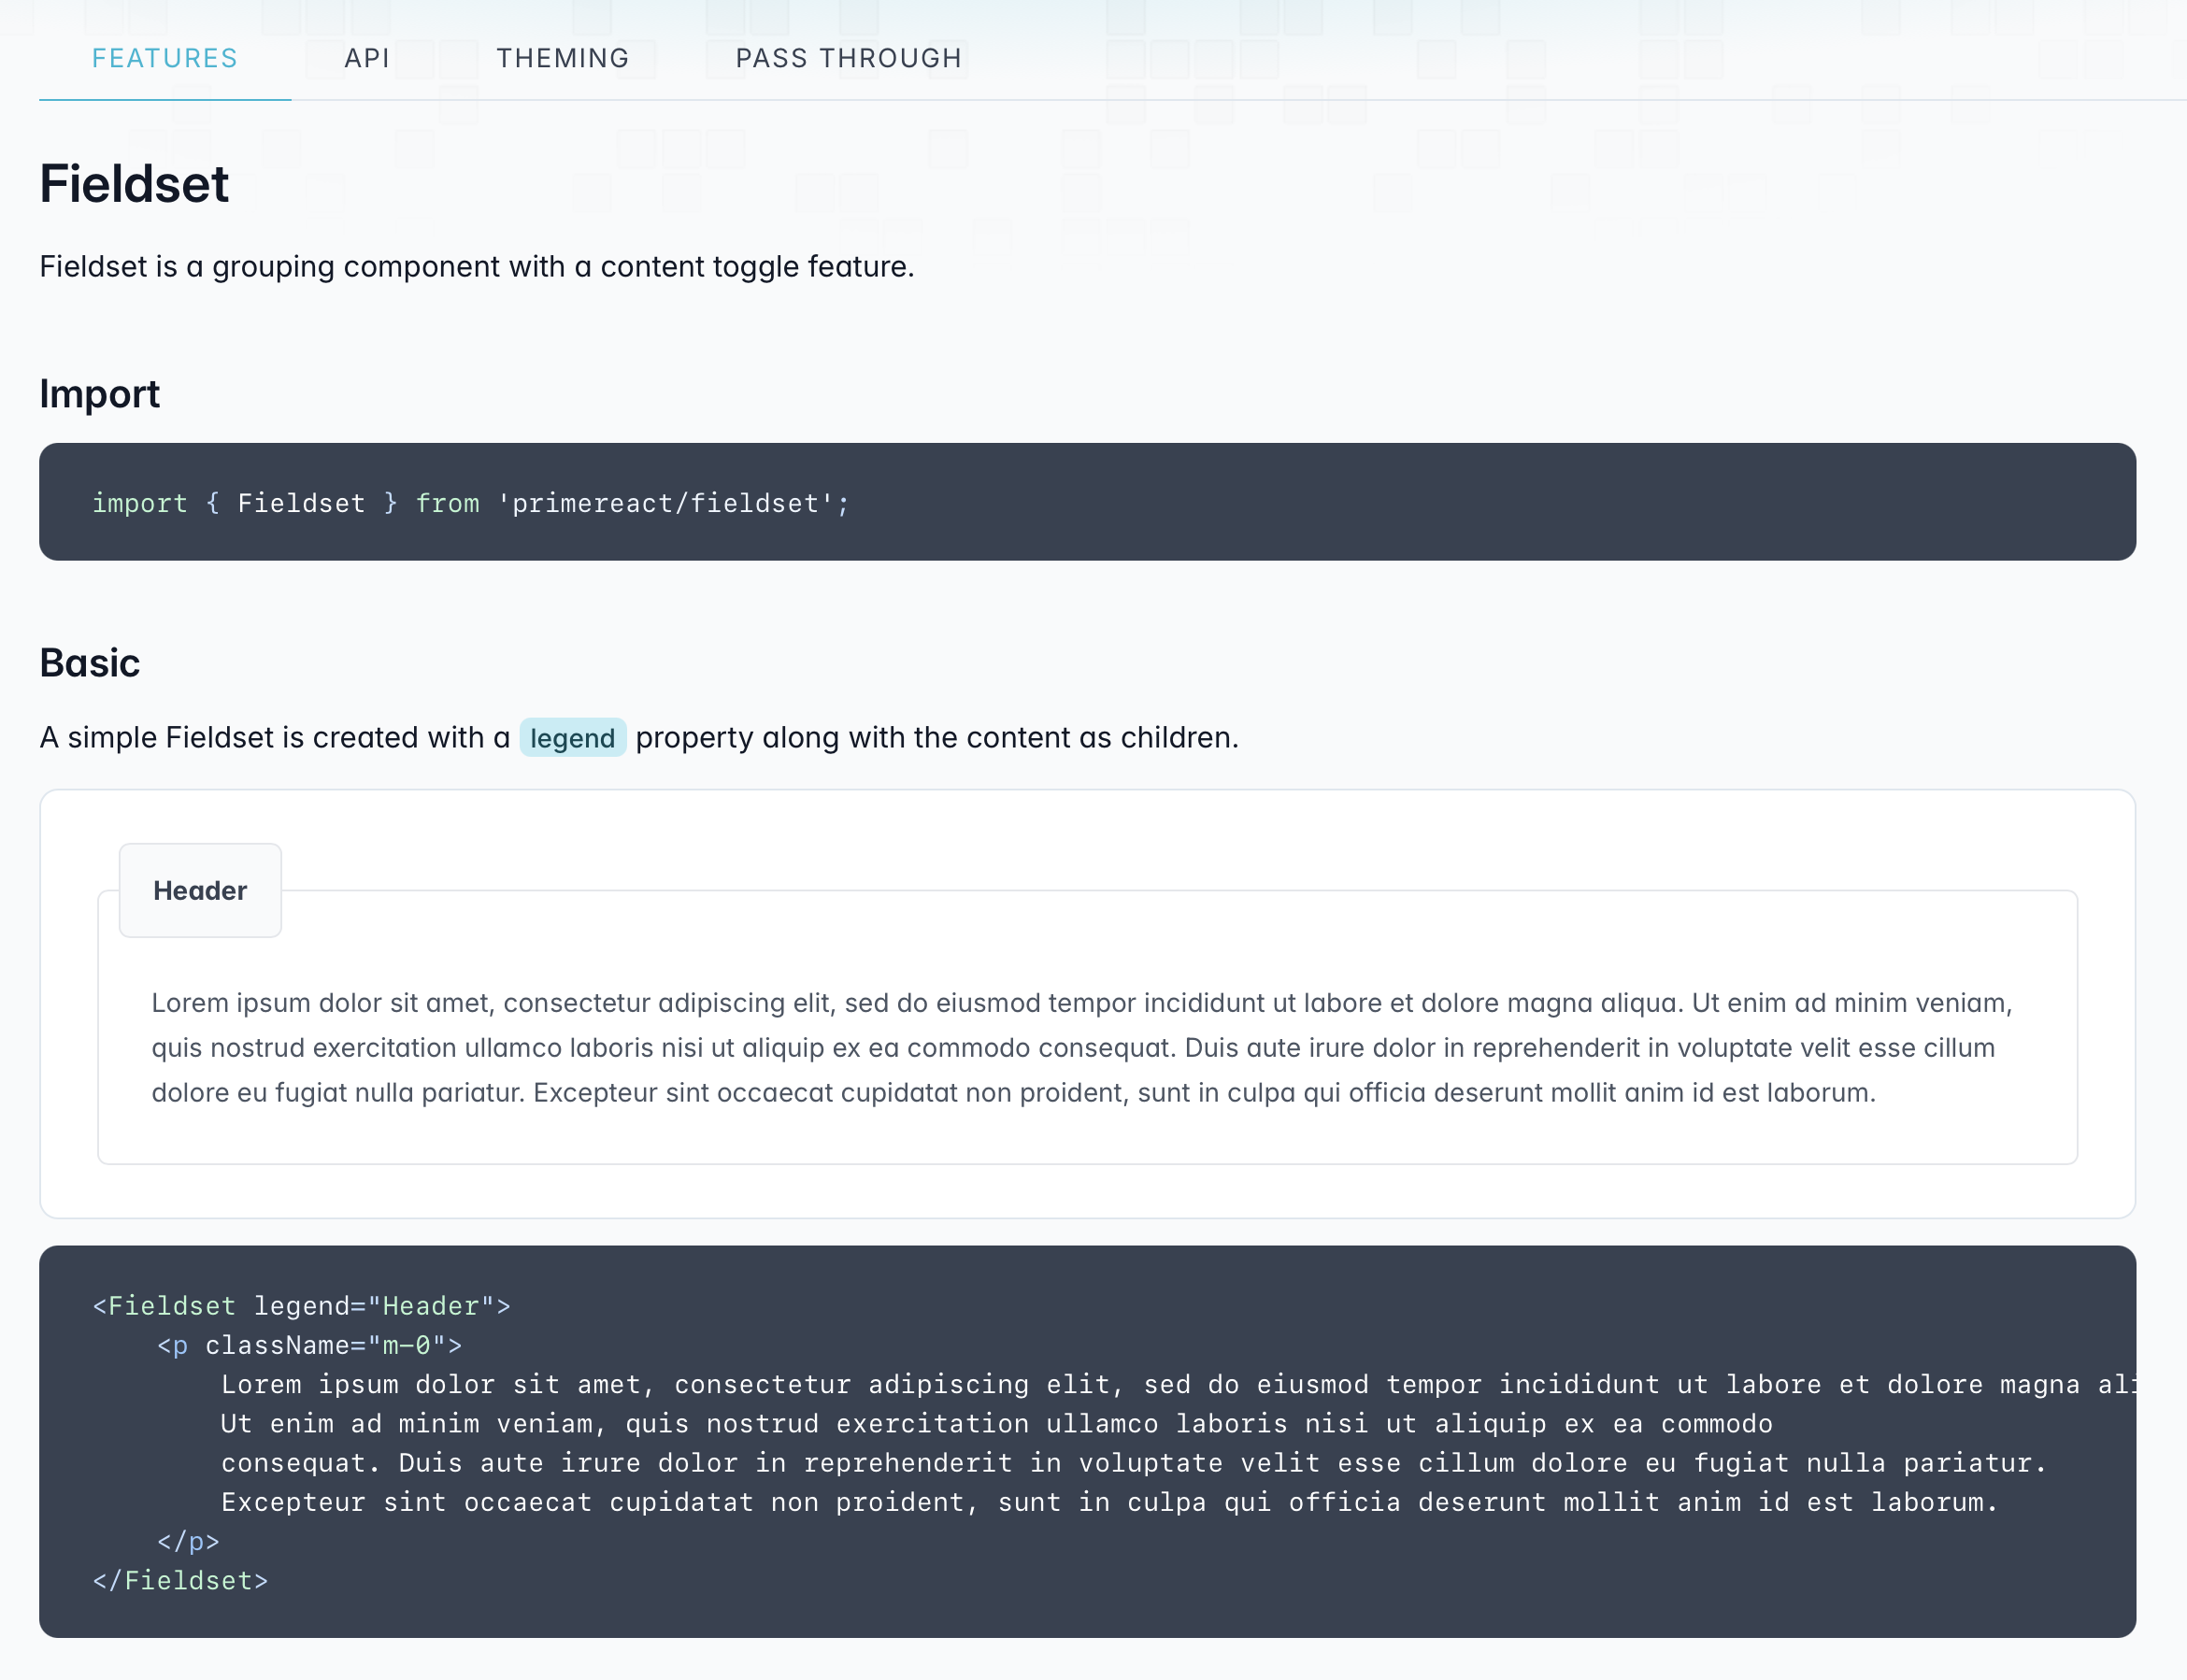
\includegraphics[width=\textwidth]{2}
		\end{figure}
	\end{minipage}
\end{frame}

\section{Code Qualität}
\begin{frame}
	\frametitle{Code Qualität}
		\begin{itemize}
			\item Probleme bei der Einrichtung von SonarQube (Unit Test Isolation)
			\item Hat geholfen Code Smells und Bad Practices zu erkennen
			\item Debugging hat 1 Woche gebraucht
			\item Unit-Tests für Backend waren nützlich
		\end{itemize}
		\begin{figure}
			\raggedright
			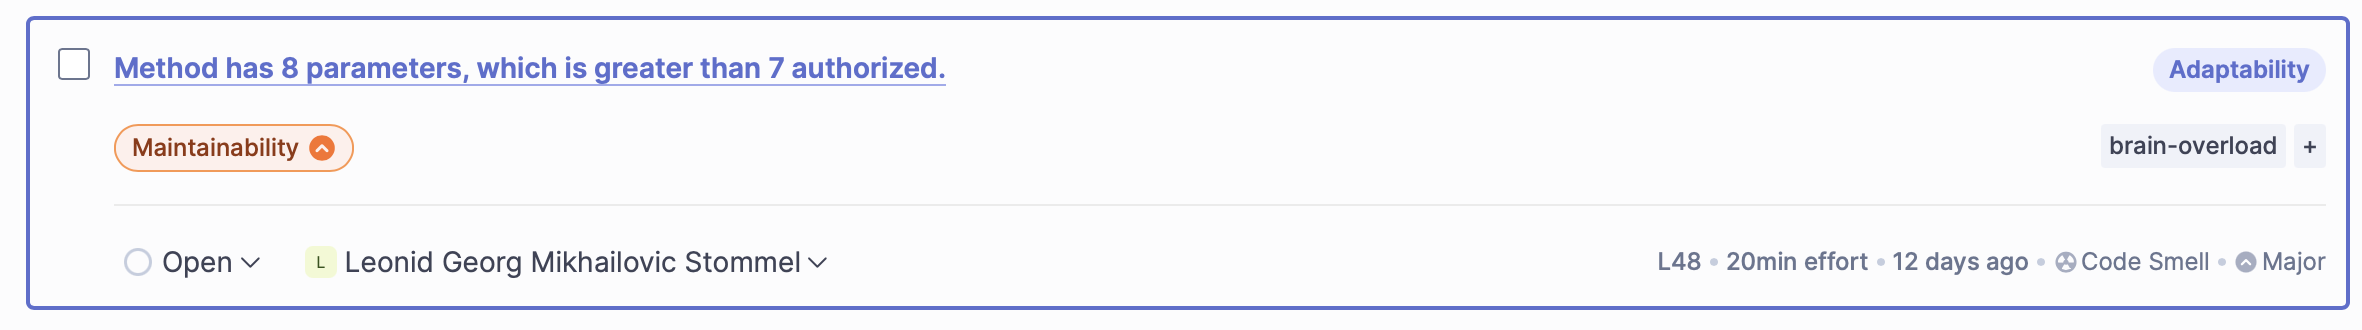
\includegraphics[width=\textwidth]{3}
		\end{figure}
\end{frame}	

\section{Fazit}
\begin{frame}
	\frametitle{Fazit}
	\begin{minipage}{0.45\textwidth}
		\begin{itemize}
			\item Herausforderungen: center a div, API Debugging , Layout
			\item Geholfen haben die React Debugging Tools
			\item Beim nächsten Mal: wieder Aufteilung in Aufgaben, Dependencies besser aufarbeiten
		\end{itemize}
	\end{minipage}
	\begin{minipage}{0.45\textwidth}
		\begin{figure}
			\raggedright
			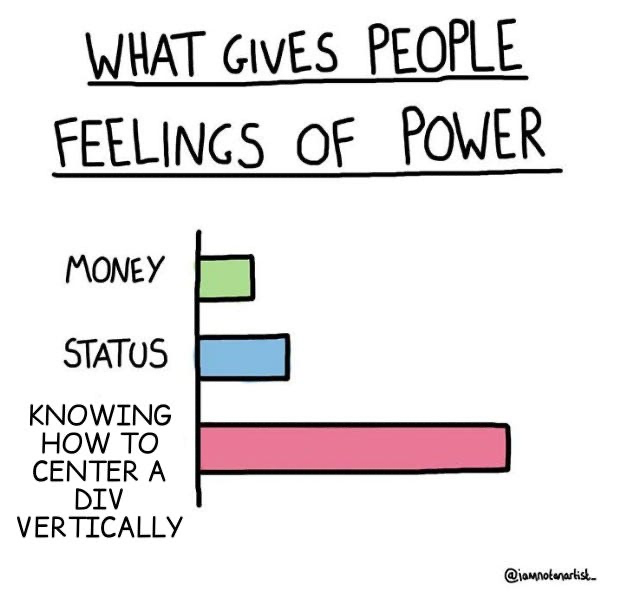
\includegraphics[width=\textwidth]{4}
		\end{figure}
	\end{minipage}
\end{frame}

\end{document}